%   %==========================================================================
%   %  Comment
%   %==========================================================================
\begin{mycomment}
    熱力学では,主に気体の熱に関する物理法則を学んでいく.
    熱力学で着目する日常的に経験する物理現象を取り上げ,熱力学でどんな現象を
    解析するのかをイメージしよう.それと同時に,熱現象に関する経験則を日常
    経験の中からピックアップする.さらに,いくつかの実験結果・法則を紹介する.
    それらから,熱力学の理論を構築していこう.
\end{mycomment}

%   %==========================================================================
%   %  Section
%   %==========================================================================
\section{熱力学的な系}
    \begin{mycomment}
        熱力学で着目する日常的に経験する物理現象を取り上げてみる.
        熱力学学習最初の教科書として,菊川芳夫 著:
        「講談社の基礎物理シリーズ3『熱力学』」(講談社)を用いる.
        この教科書は具体例が豊富でイメージしやすい.
    \end{mycomment}

    \subsection{平衡状態/非平衡状態}
    熱力学では安定した状態(\textbf{平衡状態})をあつかう.インクの拡散が進行している状態など
    の不安定な状態((\textbf{非平衡状態}))は扱えない.インクの拡散が終わり再び安定した状態
    になった場合は熱力学の対象になる.つまり,変化の前後の安定状態は熱力学の対象であるが,
    変化中の仮定は熱力学では扱えない.
    \begin{figure}[hbt]
        \begin{center}
            \includegraphicsdefault{heikou_hiheikou.pdf}
            \caption{熱力学の対象(平衡状態/非平衡状態)}
            \label{fig:heikou_hiheikou}
        \end{center}
    \end{figure}

    \subsection{熱平衡状態}
        すでに私達は学校で,物質は無数の原子や原子から構成されていることを学んでいる.
        高校では,主に化学の分野で,\textbf{アボガドロ定数} ${N}_{a}$ という巨大な数字に
        であう.
        \begin{equation}
            {N}_{A} := 6.02214179(30) \times {10}^{23} \mbox{[mol${}^{-1}$]}
        \end{equation}
        アボガドロ定数と同じくらいの原子や分子が存在して,これを1つの考察対象の系するとき,
        \textbf{巨視的(マクロ,macroscopic)}な系という.

        巨視的な系は,一定の環境や拘束の下で十分に長い時間が経過すると,系の物理的な性質
        がそれ以上変化しない平衡状態となり,温度・圧力・体積・物質量(モル数)など,巨視的な
        装置で測定される極小数の物理量によって記述できる.このような平衡状態を熱力学では,
        \textbf{熱平衡状態} という.熱平衡状態に応じて値が決まる物理量を \textbf{状態量} という.
        熱平衡状態の例として,以下がある.
        \begin{itemize}
            \item 熱平衡($\rightarrow$ \ref{sbsbsec:netsu_heikou}節参照)
            \item 相平衡($\rightarrow$\ref{sbsbsec:sou_heikou}節参照)
            \item 化学平衡($\rightarrow$\ref{sbsbsec:kagaku_heikou}節参照)
        \end{itemize}

        巨視的に見て平衡状態(変化がない状態)にある系が熱力学の対象となりうる
            \footnote{
                平衡状態であれば,熱力学で扱えない場合もあるかもしれない.
            }

        時間変化する状態を \textbf{非平衡状態} というが,熱力学では簡単には扱えない.
        通常,熱力学というばあいは平衡状態の理論を指す.非平衡状態の熱力学理論も
        構築されつつあるが,まだ安定した教科書が数少ない.あっても内容が高度である.

        熱力学が対象とする系は,均質な系(あるいは,均質な部分系)である.
        また,系の組成としては,一種の原子・分子からなる単一系や,数種類の原子・分子からなる
        混合系が考えられる
            \footnote{
                単一系の原子の例として,水(\ce{H2O})を分解してできた水素(\ce{H2})や酸素(\ce{O2})がある.
                単一系の分子の例は,先の水(\ce{H20})やアンモニア(\ce{NH3})がある.
                数種類の分子からなる混合系は空気(酸素\ce{O2}・窒素\ce{N2}・アルゴン\ce{Ar}・その他)
                がある.牛乳とかスポーツドリンクなどもへ好状態にある混合系といえるだろう.
            }.

        \subsubsection{熱平衡}\label{sbsbsec:netsu_heikou}
        高温と低温の2つの物体を接触させてその状態を保ち,十分に時間が経過すると,この2つの
        物体の温度が等しくなり,温度が一定になる.この温度が一定にある状態を \textbf{熱平衡状態} にあるという.
        \begin{figure}[hbt]
            \begin{center}
                \includegraphicsdefault{netsu_heikou.pdf}
                \caption{熱平衡(物体の接触)}
                \label{fig:netsu_heikou}
            \end{center}
        \end{figure}

        高温の物体はいくらか温度が下がり,低温の物体は温度が上がる.
        \begin{figure}[hbt]
            \begin{center}
                \includegraphicsdefault{netsu_heikou_graph.pdf}
                \caption{熱平衡(温度推移のグラフ)}
                \label{fig:netsu_heikou}
            \end{center}
        \end{figure}

        \subsubsection{相平衡}\label{sbsbsec:sou_heikou}
        水を沸騰させてシリンジにピストンで吸い込み,ゴム栓をする.
        このとき,空気が入らないようにピストンを調整する.シリンジの中に
        封入された物質系は,水分子からなる液体の均質な系である.

        その後,ピストンを押すと内部の水が沸騰して,その一部が水蒸気に変わる.
        この状態を保つようにピストンをストッパーで留めておく
            \footnote{
                つまり,ピストン内部の圧力を高いままにしておく.
            }.
        このシリンジ内部の系は同じ水分子からなる単一系だけど,液体(水)と
        気体(水蒸気)という異なる2つの均質な部分系に分かれている.
        これを \textbf{相平衡} という.
        \begin{figure}[hbt]
            \begin{center}
                \includegraphicsdefault{sou_heikou.pdf}
                \caption{相平衡:熱湯を圧縮}
                \label{fig:netsu_heikou}
            \end{center}
        \end{figure}

        液体(水)と気体(水蒸気)が共存し,相平衡になるときの圧力は,温度によって決まる.
        温度が低いほど相平衡になる圧力は小さく,温度が高いほど相平衡の圧力は高くなる.
        この相平衡となる圧力を \textbf{飽和蒸気圧} という.
        飽和蒸気圧を温度の関数として表したグラフを \textbf{蒸気圧曲線} という.
        \begin{figure}[hbt]
            \begin{center}
                \includegraphicsdefault{sou_heikou_graph.pdf}
                \caption{水の蒸気圧曲線}
                \label{fig:sou_heikou_graph}
            \end{center}
        \end{figure}

        \subsubsection{化学平衡}\label{sbsbsec:kagaku_heikou}
        一定の温度に保たれた容器の中で,窒素・水素・アンモニアの気体を混合する.
        窒素分子\ce{N2}が反応してアンモニア分子\ce{NH3}が生成され,逆に,アンモニア分子が分解して
        窒素分子と水素分子が生成される.この仮定の化学反応式は
        \begin{equation}
            \ce{N2} + 3\ce{H2} \ce{<-->} 2\ce{NH3}
        \end{equation}
        となる.しばらくすると,アンモニアの生成される反応速度と分解される反応速度が等しくなり,
        窒素・水素・アンモニアの物質量が一定の状態になる.これを \textbf{化学平衡} という.

        このとき,窒素・水素・アンモニアのモル濃度をそれぞれ[\ce{N2}]・[\ce{H2}]・[\ce{NH3}]と表せば,
        次の関係式が成り立つ.
        \begin{equation}
            \frac{[{\ce{NH2}}^{2}]}{[\ce{N2}][\ce{H2}]} = {K}_{c} = \mbox{一定}.
        \end{equation}
        ここで,${K}_{c}$は温度で決まる定数である.この関係式を \textbf{質量作用の法則} という.

        \subsection{準静的過程}
        変化中の状態は熱力学では扱えないのだが,その変化を少しずつ微小変化させる場合,つまり,その微小変化
        の前後では状態が変化したことを認識できないレベルで状態を少しずつ変化させる場合は熱力学で扱える場合がある.
        このような微小変化を連続させて状態変化を観測するとき,この微小変化のことを \textbf{準静的過程} という.

        例えば,ピストンの内部の物質を圧縮する場合,急激に圧力をかけて体積を小さくする場合は変化が大きいので
        熱力学で扱えない.しかし,敷居を微小変位させて,とてもゆっくり
            \footnote{
                無限回の微小移動,あるいは,無限の時間をかけてゆっくりと移動させるイメージ.
            }
        変化させた場合は,一回の微小変化の前後では変化がないため,熱力学で扱える.この無限回微小変化の繰り返し
        は準静的過程の一種である
            \footnote{
                0歳と80歳とで外面を比べると大きく違うが,その過程は準静的過程である.
                徐々に太っていく様子も準静的過程といえる.
                変化していないように見えるけど,実は変化している.だから,"準"静的過程という.
                完全に動いていない(静的)わけでもなく,だからといって変化しているようには見えない.
                準静的過程はとても恐ろしい.
            }.
        \begin{figure}[hbt]
            \begin{center}
                \includegraphicsdefault{junseiteki_katei.pdf}
                \caption{準静的過程の例}
                \label{fig:junseiteki_katei}
            \end{center}
        \end{figure}



\section{状態量}
        \subsection{熱力学で扱う変数(状態量)}
        単一の原子または分子からなる均質な系の熱平衡状態は,通常,温度$T$,体積$V$,物理量$n$によって
        特定することができる.温度または体積の変わりに圧力]$p$を用いることもできる.
        これらの物理量は \textbf{状態量} である.

        状態量の測定に用いる装置は巨視的であるため,測定値や測定に要する時間も巨視的なスケールになる.

        \begin{itembox}[l]{熱力学で扱われる単位の例}
            [L](リットル)/[m${}^{3}$](立方メートル)/[\circC](度)/[mol](モル)/
            [kg](キログラム)/[Pa](パスカル)/[N/m${}^{2}$](ニュートン毎平方メートル)/
            [s](秒,あるいは,分や時間)
        \end{itembox}

        ややこしいことに,仕事$W$と熱量$Q$は状態量ではない.

        \subsection{示強変数と示量変数}
            熱平衡状態にある均質な系を部分系に分けた場合,その各々の部分系も熱平衡状態である.
            分かれた部分系を再び合成しても,何の変化も生じない.このとき,部分系の物質量
            (${n}_{1}$,${n}_{2}$,$\cdots$)に比例して変化するか,あるは分割前のもとの系と
            同じであるか,のいずれかである.例えば,体積は分割するとその分割の大きさ(物質量)に比例
            して小さくなる.他方で,温度や圧力は分割しても変化はない.体積のように,
            物質量に比例して変化する量のことを \textbf{示量的} という.温度や圧力のように分割しても
            変化しない量を \textbf{示強的} という.また,体積や温度や圧力などを変数化して式として
            現すとき,体積などの分割したら変化する示量的な変数のことを \textbf{示量変数} といい,
            温度や圧力などの分割しても変化しない示強的な変数のこと \textbf{示強変数} という.
            \begin{figure}[hbt]
                \begin{center}
                    \includegraphicsdefault{shikyouhensu_siryohensu.pdf}
                    \caption{示強変数と示量変数の例}
                    \label{fig:shikyouhensu_siryohensu}
                \end{center}
            \end{figure}

        \begin{mysmallsec}{インク溶液の状態量}
            ビーカー内の水にインクを数滴垂らしてしばらく放置すると,インクは拡散してインクの密度は均一になる.
            この水とインクの均質な混合系の状態量は,体積$V$と水のモル数$n$(またはの密度($n/V$))および温度$T$である.

            均一になった後に,ビーカーに仕切りを入れて水と混合系を均質な2つの部分系にわけると,2つの部分系の
            温度と水とインクの密度はそれぞれ等しい.仕切りを取り除いて2つの部分系を合わせても,温度と水とインクの
            密度に変化はない.したがって,温度と水のインクの密度は「示強的」である.

            \begin{figure}[hbt]
                \begin{center}
                    \includegraphicsdefault{netsu_shikyo_siryo.pdf}
                    \caption{インク溶液の状態量}
                    \label{fig:netsu_shikyo_siryo}
                \end{center}
            \end{figure}
        \end{mysmallsec}

\section{環境と拘束}
    \subsection{孤立系(孤立した系; isolated system)}
        物質も通さず,熱も通さず,形も変化しない容器内部の系を \textbf{孤立系} という.
        当然,外部からエネルギーや仕事の供給もない.外からいかなる影響も受けないし,
        逆に外に対していかなる影響も及ぼさない.

    \subsection{断熱系}
        外界との熱のやりとりができない系を \textbf{断熱系} という.

    \subsection{閉鎖系(閉じた系; closed system)}
        物質を通さない系のことを \textbf{閉鎖系} という.熱やエネルギーのやり取りは可能である.

    \subsection{開放系(開いた系; opened system)}
        物質も通し,熱も通し,エネルギーや仕事のやり取りも可能な系を \textbf{開放系} という.
        \begin{figure}[hbt]
            \begin{center}
                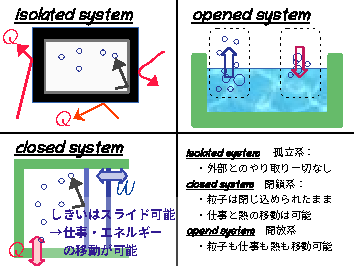
\includegraphics[keepaspectratio, width=7.5cm,height=6.9cm,clip]{neturikigaku_kankyo1.pdf}
                \caption{系の分類}
                \label{fig:neturikigaku_kankyo1}
            \end{center}
        \end{figure}

    \subsection{外界}
        着目している毛糸直接または間接的に接していて,熱や仕事,物質をやり取りする物質系を \textbf{外界} という.

    \subsection{環境}
     考察対象となる熱力学の系が置かれた周囲の状況のうち,
     室温や大気圧,熱湯(熱源)といった外界の条件をさして,これらを \textbf{環境} という.

    \subsection{拘束}
        考察対象となる熱力学の系が置かれた周囲の状況のうち,
        容器の壁やしきり,ピストンやピストンのストッパーといった,形状や体積および物質量を決める拘束条件,及び,
        断熱材や半透膜といった熱や物質の透過性を決める境界の性質,これらを \textbf{拘束} という.

    \subsection{環境と拘束}
        巨視的な系の熱平衡状態は,環境と拘束の下で,実現している.環境や拘束の変化に応じて,
        系の熱平衡状態は変化する.

    \subsection{可逆変化・非可逆変化}
        状態変化させた後で,対象とする系とその外界も含めてもとの状態に戻せる変化のこと
        を \textbf{可逆変化} という.系だけがもとに戻っ多としても,可逆変化とはいわない.
        逆に,状態を戻せない変化のことは,\textbf{非可逆変化} という.

    \subsection{断熱環境:断熱ポットの中の熱湯}
        ポットの内部には,水蒸気と空気の混合系(気体)と水の単一系(液体)の2つの部分系からなっている.
        それぞれの部分系は均質である.ポットは閉じていて,形状が固定されていることから,系の物質量と体積は
        一定に保たれている.系は熱を通さない材質の壁(\textbf{断熱壁})で囲まれていて,ポットの外部の大気の
        熱のやり取りができない.そのため,系の温度は外部の温度に影響されずに,一定の温度に保たれている.
        一方,2つの部分系(水と水蒸気・空気)の間には仕切りがなく,熱や物質を自由にやり取りできる.

        断熱ポット全体を見れば,孤立系である.内部の水と水蒸気と空気に着目すると,相互に粒子やエネルギーの
        やり取りが行えるため,個々の水と水蒸気は開放系である.
        \begin{figure}[hbt]
            \begin{center}
                \includegraphicsdefault{neturikigaku_danetu_pot.pdf}
                \caption{断熱ポット}
                \label{fig:neturikigaku_danetu_pot}
            \end{center}
        \end{figure}

    \subsection{透熱環境:シリンジの中に封入された気体}
        シリンジの内部は均質な気体の系である.ピストンとゴム栓で閉じていることで,気体の物質量は一定に保たれている.
        ピストンが\textbf{可動}である場合,内部の気体は膨張あるいは収縮ができて,体積は変化する.ピストンをストッパー
        で固定する場合は,気体の体積を一定にする拘束が加わる.系の熱を通す材質の壁(\textbf{透熱壁}:シリンジとピストン)
        で囲まれており,内部の気体はシリンジの外部の大気と熱のやりとりができる.そのため,系の温度はシリンジの外部の
        温度と等しくなる.シリンジの外部の温度・圧力は,室温・大気圧に保たれている.
        \begin{figure}[hbt]
            \begin{center}
                \includegraphicslarge{netsurikigaku_toukaheki.pdf}
                \caption{透熱壁}
                \label{fig:netsurikigaku_toukaheki}
            \end{center}
        \end{figure}

    \subsection{熱源:浴槽ないの大量の熱湯の中に置かれた鉄球}
        十分多い量の熱湯の中に小さな手球をいれた系を考える.
        熱湯と鉄球は,それぞれ均質な部分系である.鉄球は変形したり傷がついたりしないものとすれば,
        この部分の体積・物理量は一定に拘束されている.熱湯は蒸発することができ,膨張することもできる
        ので,この部分系の体積と物質量に拘束はない.鉄球と熱湯は直接的に接しているため,熱のやりとりが
        あり,その結果,どちらも温度が変わる.

        熱湯の量が十分に多く,鉄球との熱のやりとりによる温度変化が認められないとき,お湯は鉄球に対して熱の
        供給源とみなせる.これを \textbf{熱源}(\textbf{熱浴})という.ただし,大気と熱のやりとりによって
        お湯は冷めていく.一定の熱の供給源として用いるためには,湯沸かし器などによって,お湯の温度を一定に
        保つ必要がある.
        \begin{figure}[hbt]
            \begin{center}
                \includegraphicslarge{netsurikigaku_netugen.pdf}
                \caption{熱源/熱浴}
                \label{fig:netsurikigaku_netugen}
            \end{center}
        \end{figure}


    \subsection{半透膜:半透膜でしきられた希薄溶液}
    ある液体に少量の物質を溶かして作った溶液を \textbf{希薄溶液} という.溶けている物質を \textbf{溶質} といい,
    溶かすために用いる液体を \textbf{溶媒} という.また,溶媒は透過するが溶質は透過しないような膜状の物質を \textbf{半透膜} という.

    ビーカー内を半透膜で2つに仕切り,片方には溶媒のみを,もう片方には溶質と溶媒を入れる.十分時間が経過した後,ビーカー内の気迫溶液の系は,
    半透膜で仕切られた溶媒と溶質の混合系と,溶媒のみ系の2つの均質な系からなる.溶質の物質量は半透膜によって片側の系(混合系)に拘束されている.
    溶質の物質量は2つの系の間で自由にやりとりができる.

    ビーカー内の希薄溶液とビーカー外の大気との境界にしきりはなく,熱や物質を自由にやり取りできる.外界の条件は室温で大気圧にある.
    \begin{figure}[hbt]
        \begin{center}
            \includegraphicsdefault{netsurikigaku_hantoumaku.pdf}
            \caption{半透膜}
            \label{fig:netsurikigaku_hantoumaku}
        \end{center}
    \end{figure}

\section{絶対温度(気温計による定義)}
    \subsection{熱力学第0法則}
        系Aと系Bが熱平衡状態にあり,系Aと系Cが熱平衡状態にあるならば,系BとCも熱平衡状態にある.
        これは経験則で,実験事実である.熱力学の理論体系の基礎になる事柄なので,
        このことを \textbf{熱力学第0法則} といわれることも多い.ただ,熱力学の第1法則と第2法則に
        比べると,この第0法則という表現は少し非公式の感じがする.しかし,大事な原則の1つである.
        \begin{figure}[hbt]
            \begin{center}
                \includegraphicsdefault{netsu_heikou_law0.pdf}
                \caption{熱平衡(\textbf{熱力学第0法則})}
                \label{fig:netsu_heikou}
            \end{center}
        \end{figure}

    \subsection{温度}
        実際,透熱壁を介して,系Bと系Cを接触させてみると,温度など状態量に変化はなく,互いに熱平衡状態に
        あることがわかる.このように,1つの系を基準にして,他の2つの系が互いに熱平衡状態にあるかどうかを,
        直接接触させることなく判断できる.この熱平衡状態の性質は,\textbf{温度計} によって温度を定めることの
        できる原理的な理由になっている.系Aを温度計とみなせば,系Bと系Cは等しい温度にあるとえる.
        \begin{figure}[hbt]
            \begin{center}
                \includegraphicslarge{netsurikigaku_ondokei.pdf}
                \caption{温度計}
                \label{fig:netsurikigaku_ondokei}
            \end{center}
        \end{figure}

        温度の目盛りを決めるには,一般に,温度計に用いる物質の熱膨張の性質を利用する.
        ほとんどの物質は温度が高くなると体積が膨張し,温度が低くなると収縮する性質を持つ.
        熱膨張とは,温度による体積の膨張のことのことである.

        温度計に用いる物質は何でも良い.昔は(昭和,平成初期),実用的には水銀やアルコールが使われていた.
        水の凝固点(0[\circC])のときの物質の体積を${V}_{0}=$,また,
        水の沸点(100[\circC])のときの物質の体積${V}_{100}=$として,
        その差${V}_{100}-{V}_{0}$を100等分して目盛りを作る.
        このように考えた場合,温度$t$体積$V$の関数として現すことができて($t=t(V)$),
        \begin{equation}
            t(V) := 100 \times \frac{V-{V}_{0}}{{V}_{100}-{V}_{0}}
        \end{equation}
        とかける.
        逆に,温度が分かれば,体積もわかる.

    \subsection{絶対温度}
        気体は,十分に希薄でれば,その体積の膨張率は一定とみなせる.
        \begin{align}
            V &= {V}_{0} + \frac{{V}_{0}}{273.15}t  \notag \\
              &= {V}_{0}\left( 1 + \frac{1}{273.15}t \right) \notag \\
              &= {V}_{0}\left(  \frac{273.15 + t}{273.15} \right)
        \end{align}
        シャルルの法則の一例である.

        ここで,
        \begin{equation}
            T := 273.15 + t
        \end{equation}
        となる温度を新たに定義する.これを \textbf{気体温度計による絶対温度} という.すると,
        \begin{equation}
            V(T) = {V}_{0} \frac{T}{273.15} = \frac{{V}_{0}}{273.15}T
        \end{equation}
        となり,単純な比例の式になった.
